%%%%%%%%%%%%%%%%%%%%%%%%%
% ggF only selection results
%%%%%%%%%%%%%%%%%%%%%%%%%


\begin{figure}[htp]
\centering
	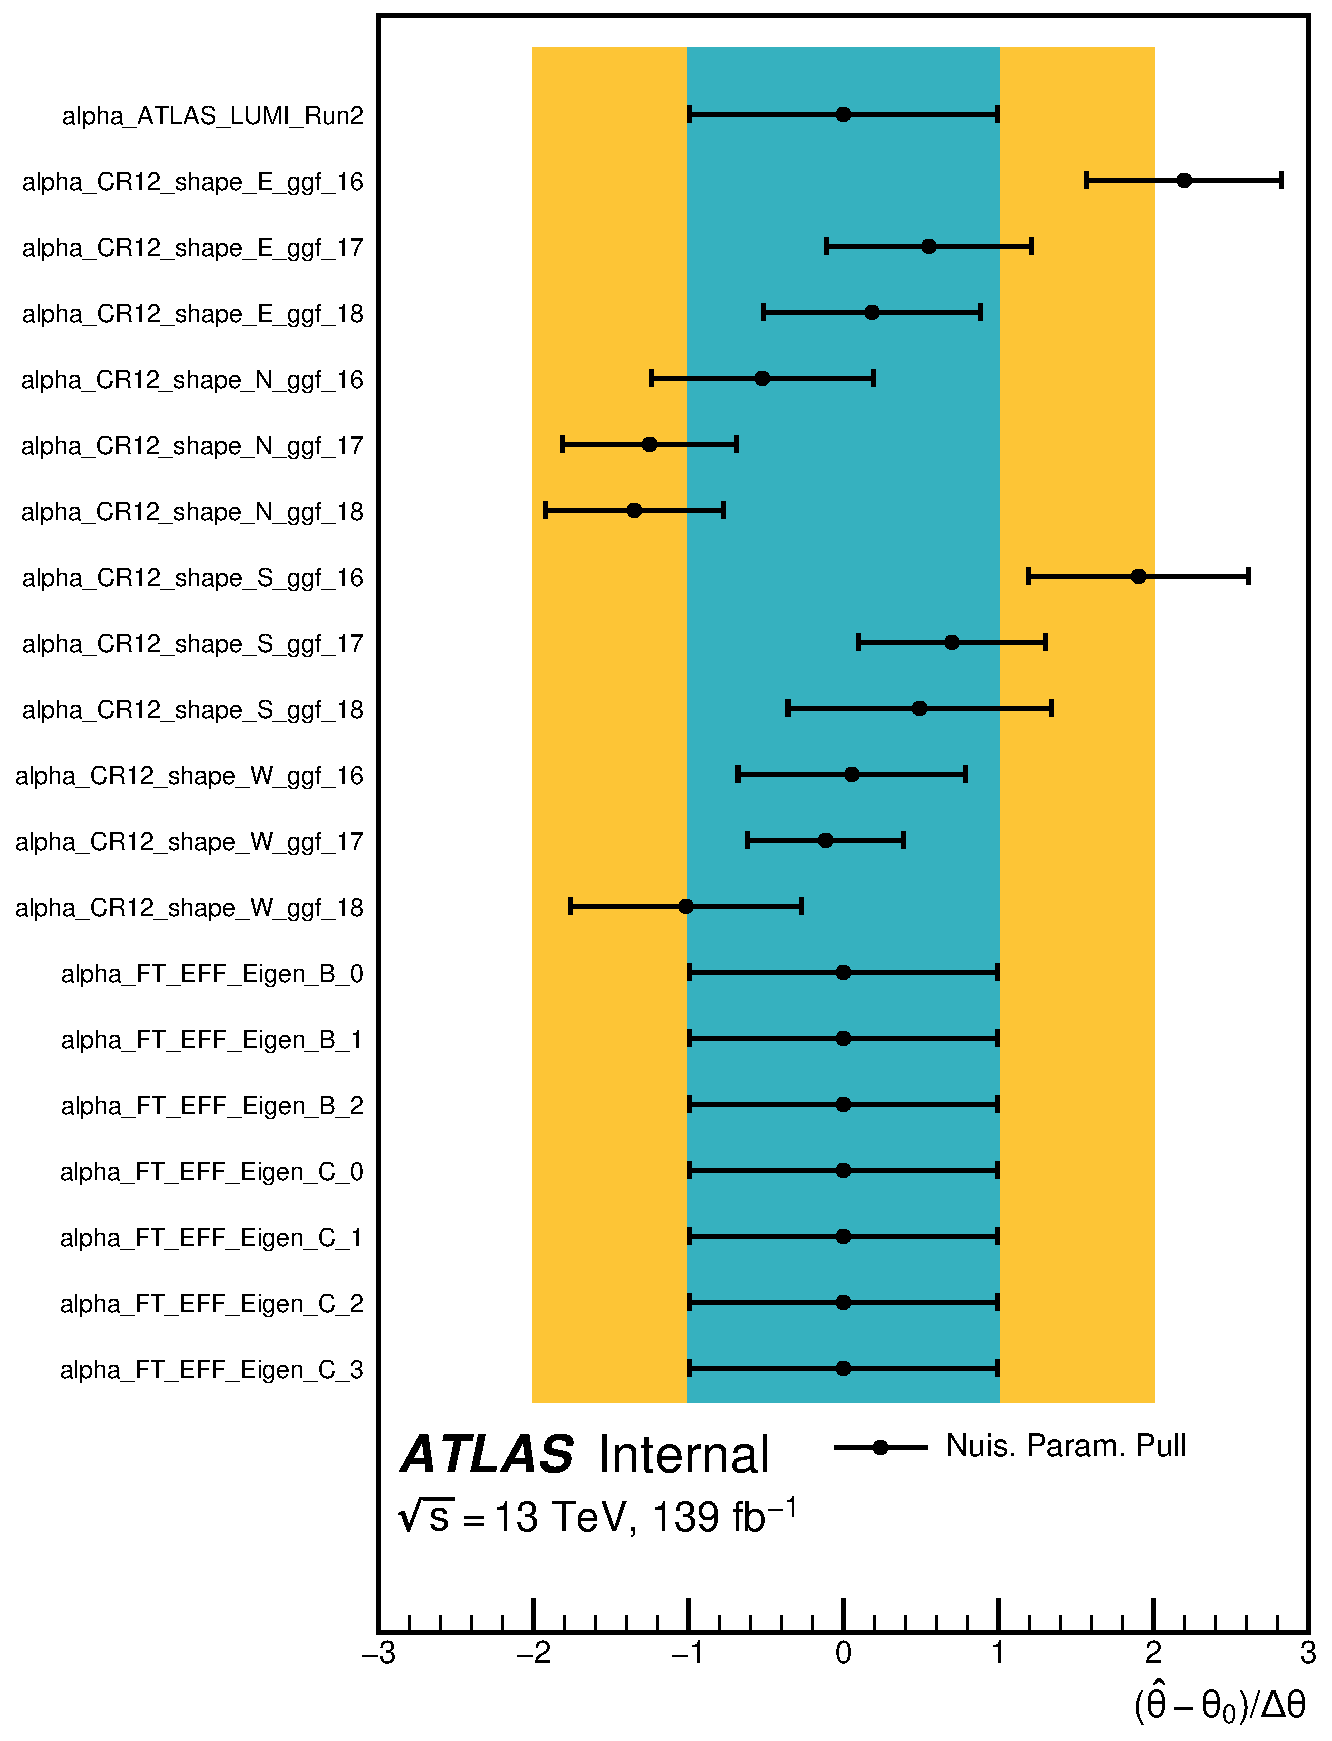
\includegraphics[width=0.33\textwidth]{\figDir/\corrscheme/pulls/quickstats_pulls_correlated_fullsyst_unblind_bkg_new_deta_Xhh_3x2_res_p09_samps_ggf_pd_ggf_161718_mod_kl_1/quickstats_pulls_correlated_fullsyst_unblind_bkg_new_deta_Xhh_3x2_res_p09_samps_ggf_pd_ggf_161718_mod_kl_1.00_k2v_1.00_k1v_1.00_b_only_rank_0001_to_0081_1-1.pdf}
	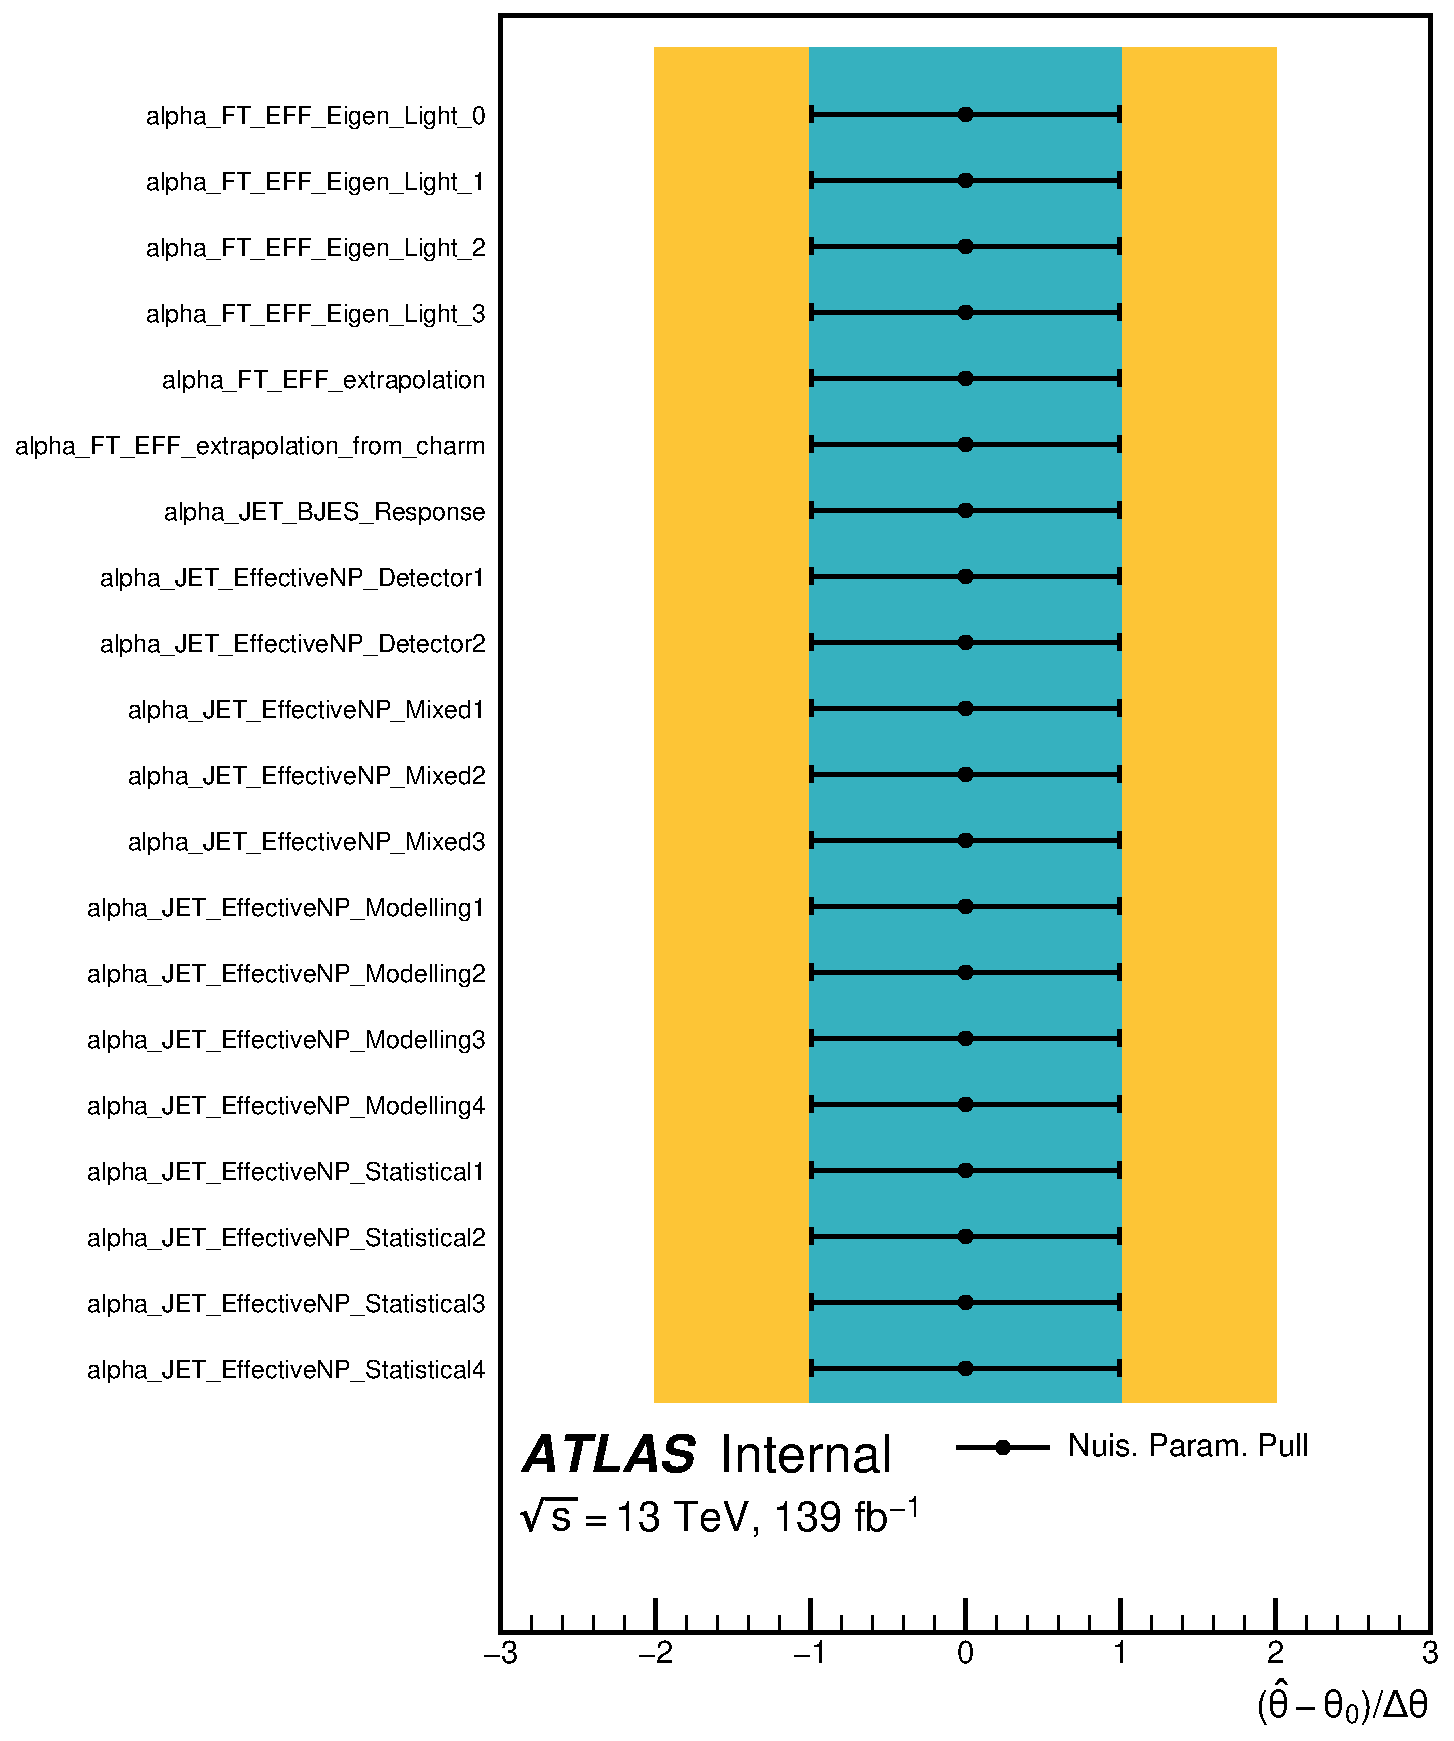
\includegraphics[width=0.33\textwidth]{\figDir/\corrscheme/pulls/quickstats_pulls_correlated_fullsyst_unblind_bkg_new_deta_Xhh_3x2_res_p09_samps_ggf_pd_ggf_161718_mod_kl_1/quickstats_pulls_correlated_fullsyst_unblind_bkg_new_deta_Xhh_3x2_res_p09_samps_ggf_pd_ggf_161718_mod_kl_1.00_k2v_1.00_k1v_1.00_b_only_rank_0001_to_0081_2-2.pdf} \\
	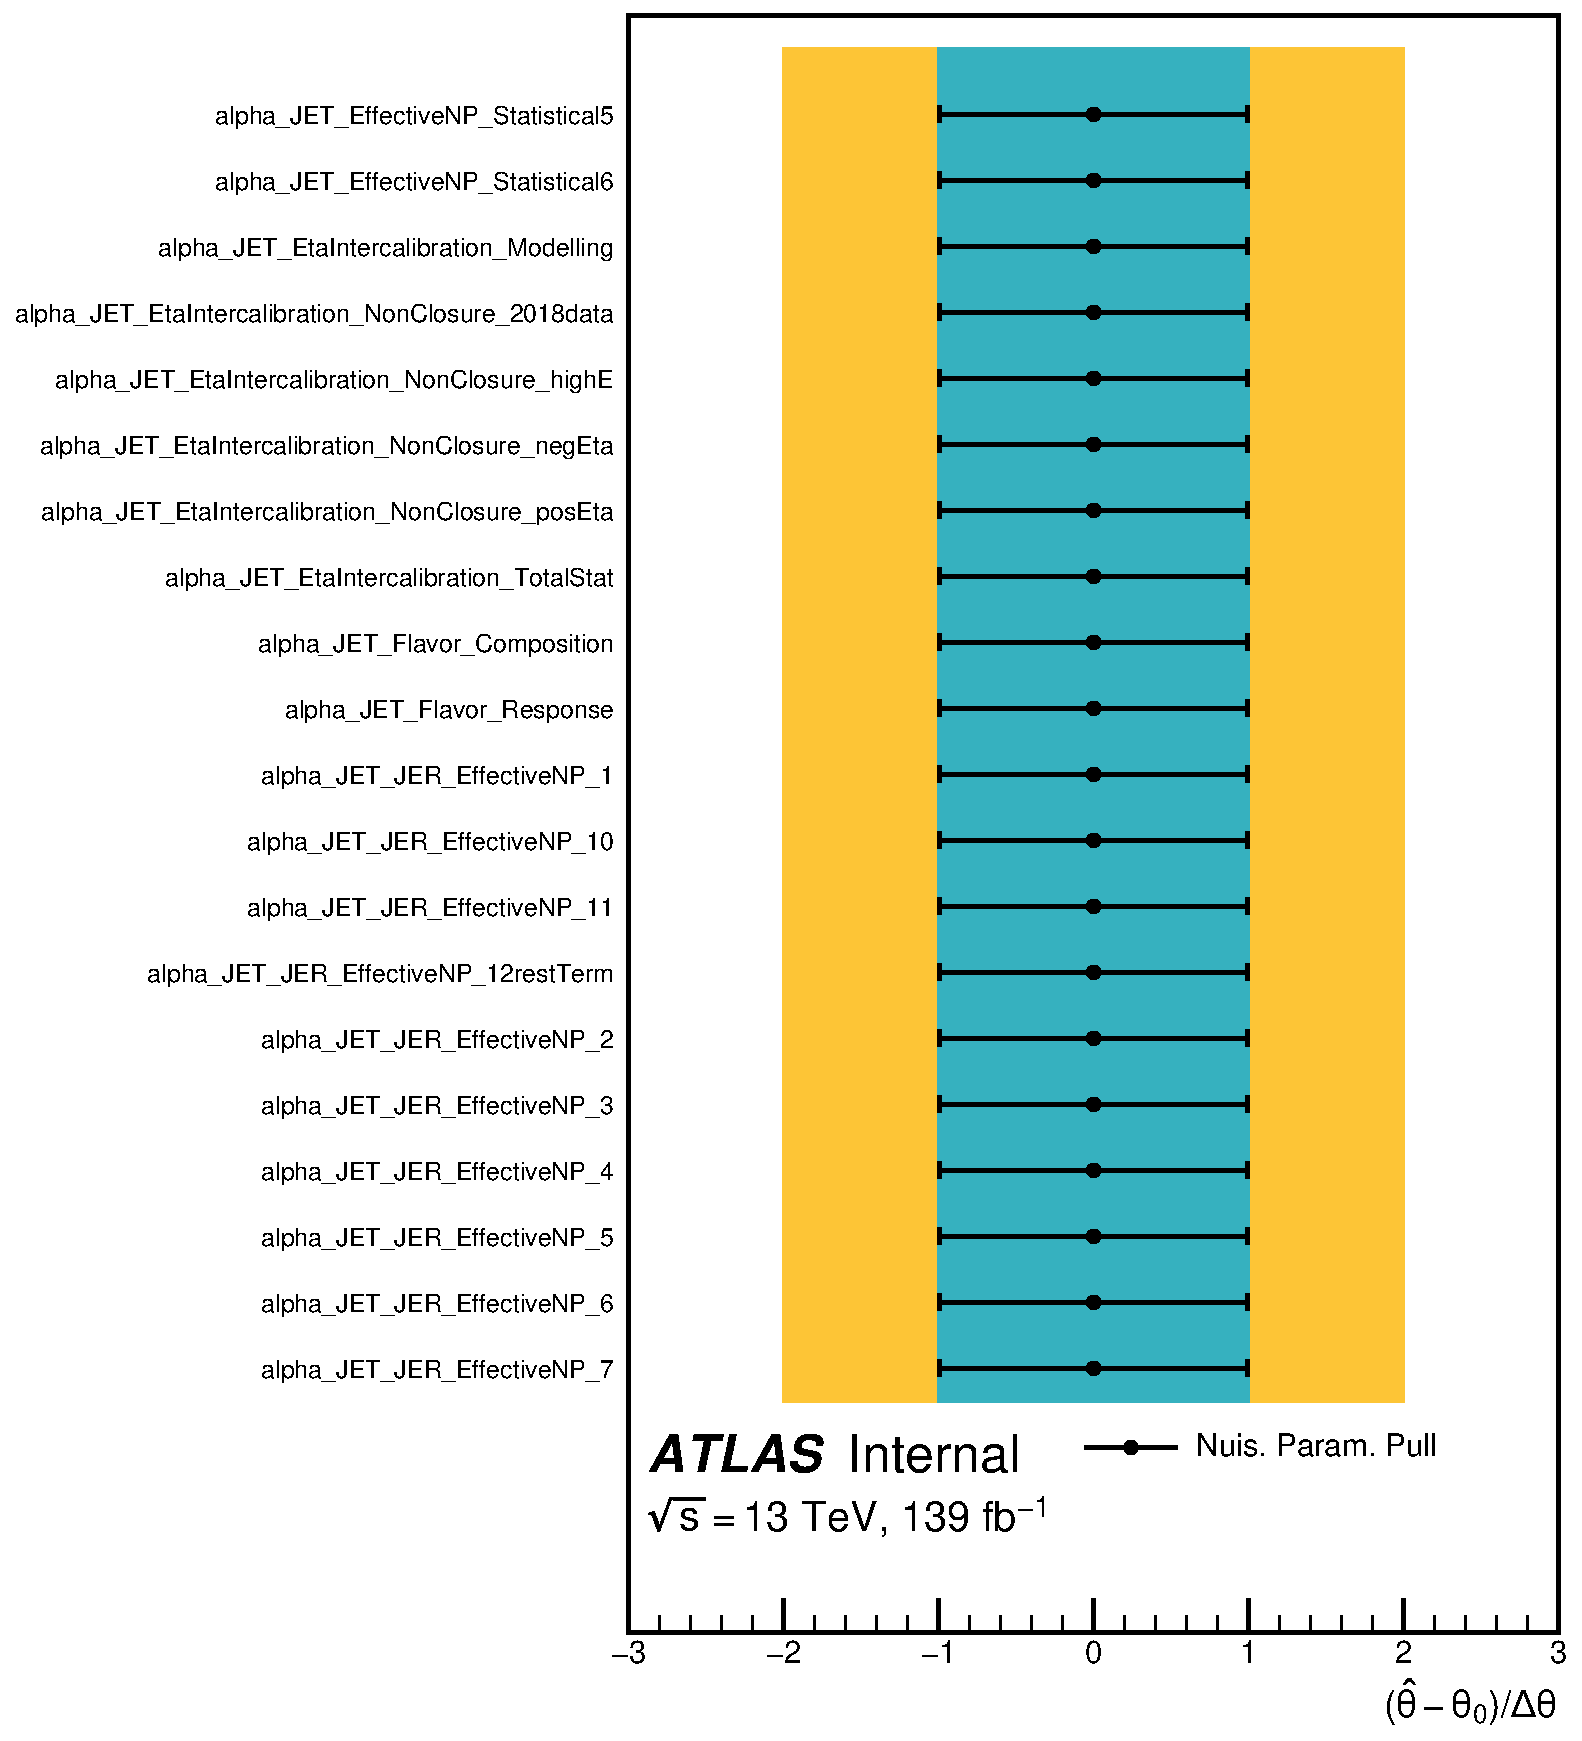
\includegraphics[width=0.33\textwidth]{\figDir/\corrscheme/pulls/quickstats_pulls_correlated_fullsyst_unblind_bkg_new_deta_Xhh_3x2_res_p09_samps_ggf_pd_ggf_161718_mod_kl_1/quickstats_pulls_correlated_fullsyst_unblind_bkg_new_deta_Xhh_3x2_res_p09_samps_ggf_pd_ggf_161718_mod_kl_1.00_k2v_1.00_k1v_1.00_b_only_rank_0001_to_0081_3-3.pdf}
	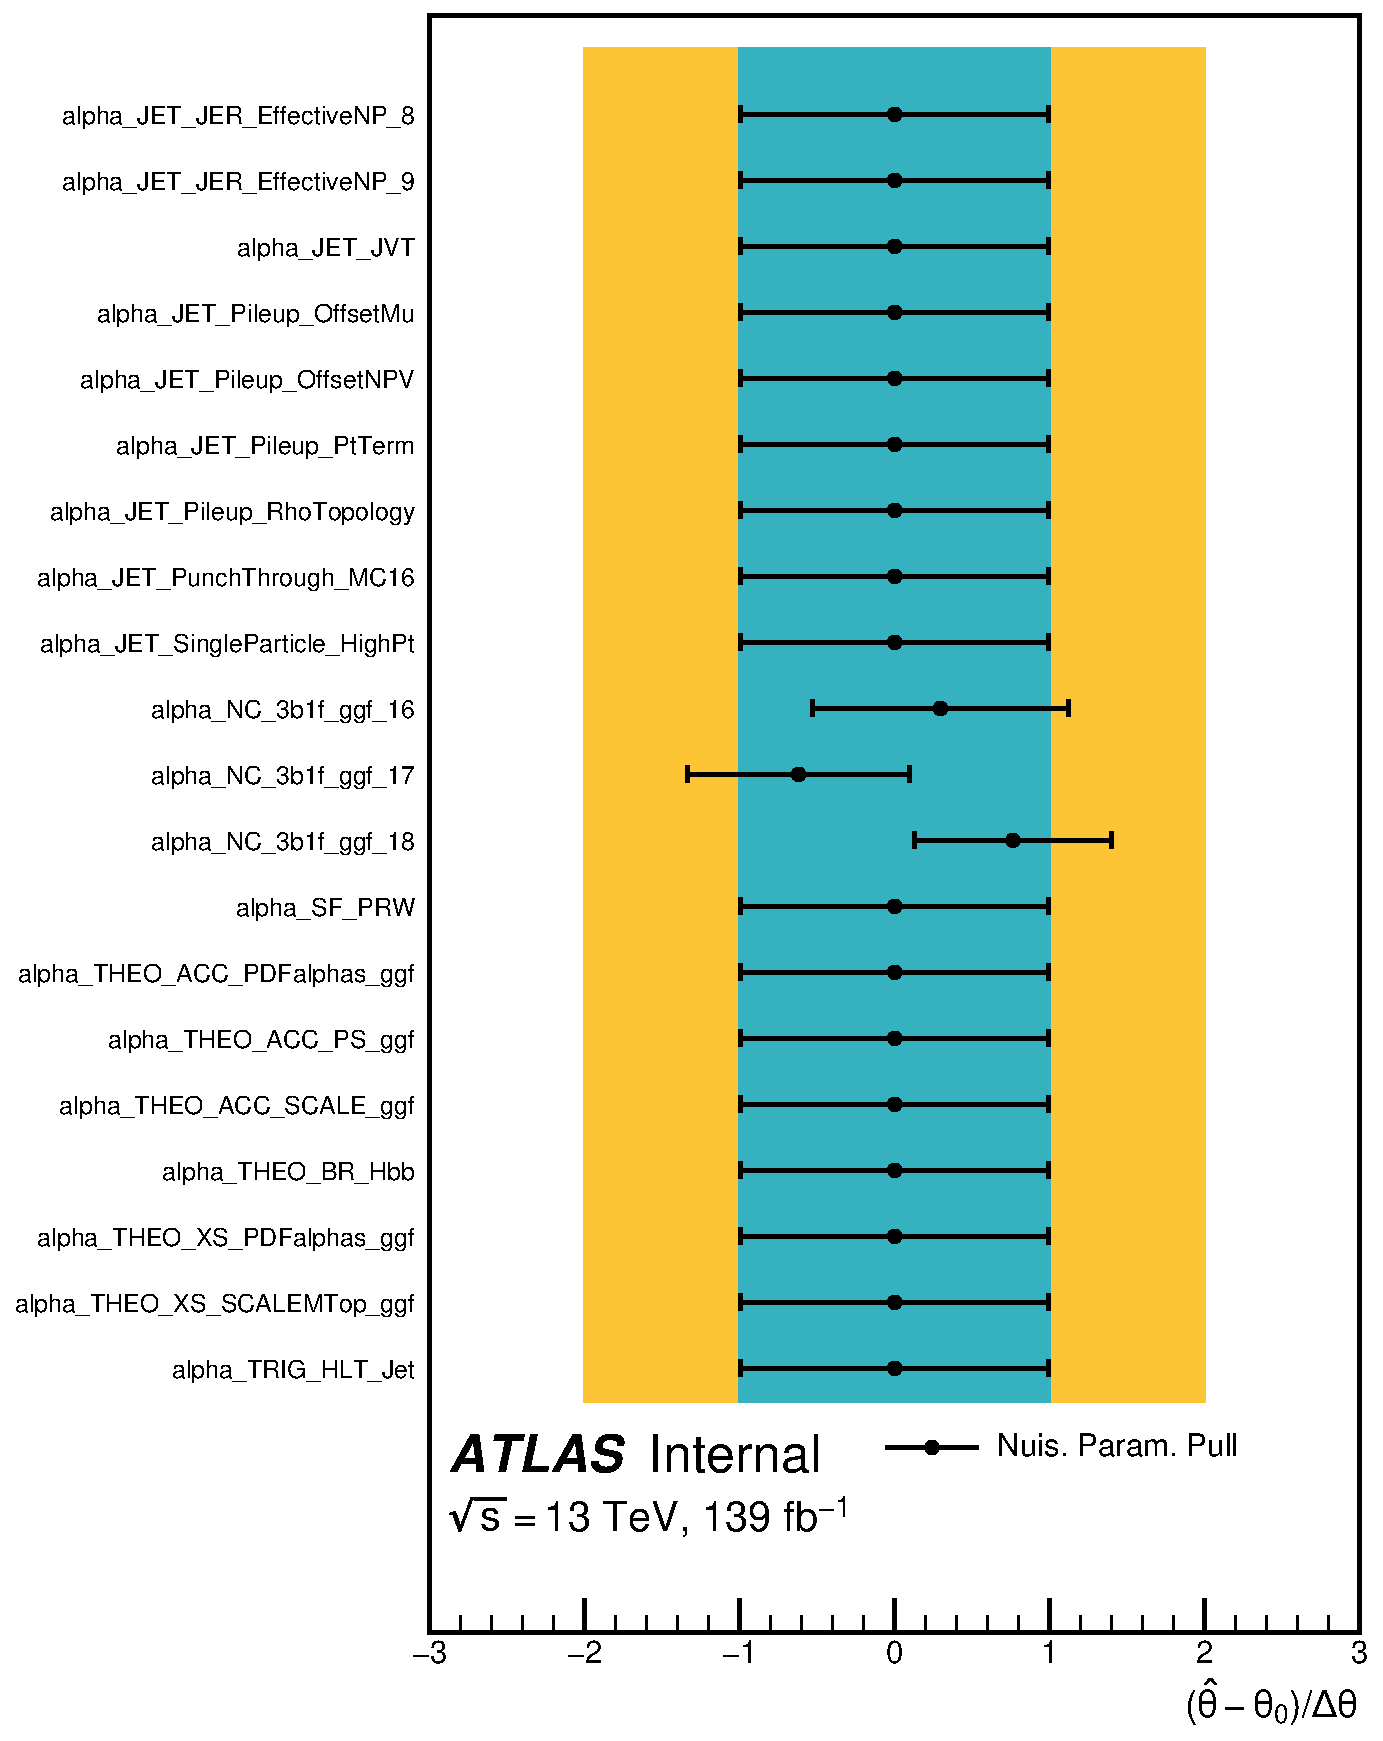
\includegraphics[width=0.33\textwidth]{\figDir/\corrscheme/pulls/quickstats_pulls_correlated_fullsyst_unblind_bkg_new_deta_Xhh_3x2_res_p09_samps_ggf_pd_ggf_161718_mod_kl_1/quickstats_pulls_correlated_fullsyst_unblind_bkg_new_deta_Xhh_3x2_res_p09_samps_ggf_pd_ggf_161718_mod_kl_1.00_k2v_1.00_k1v_1.00_b_only_rank_0001_to_0081_4-4.pdf} \\
	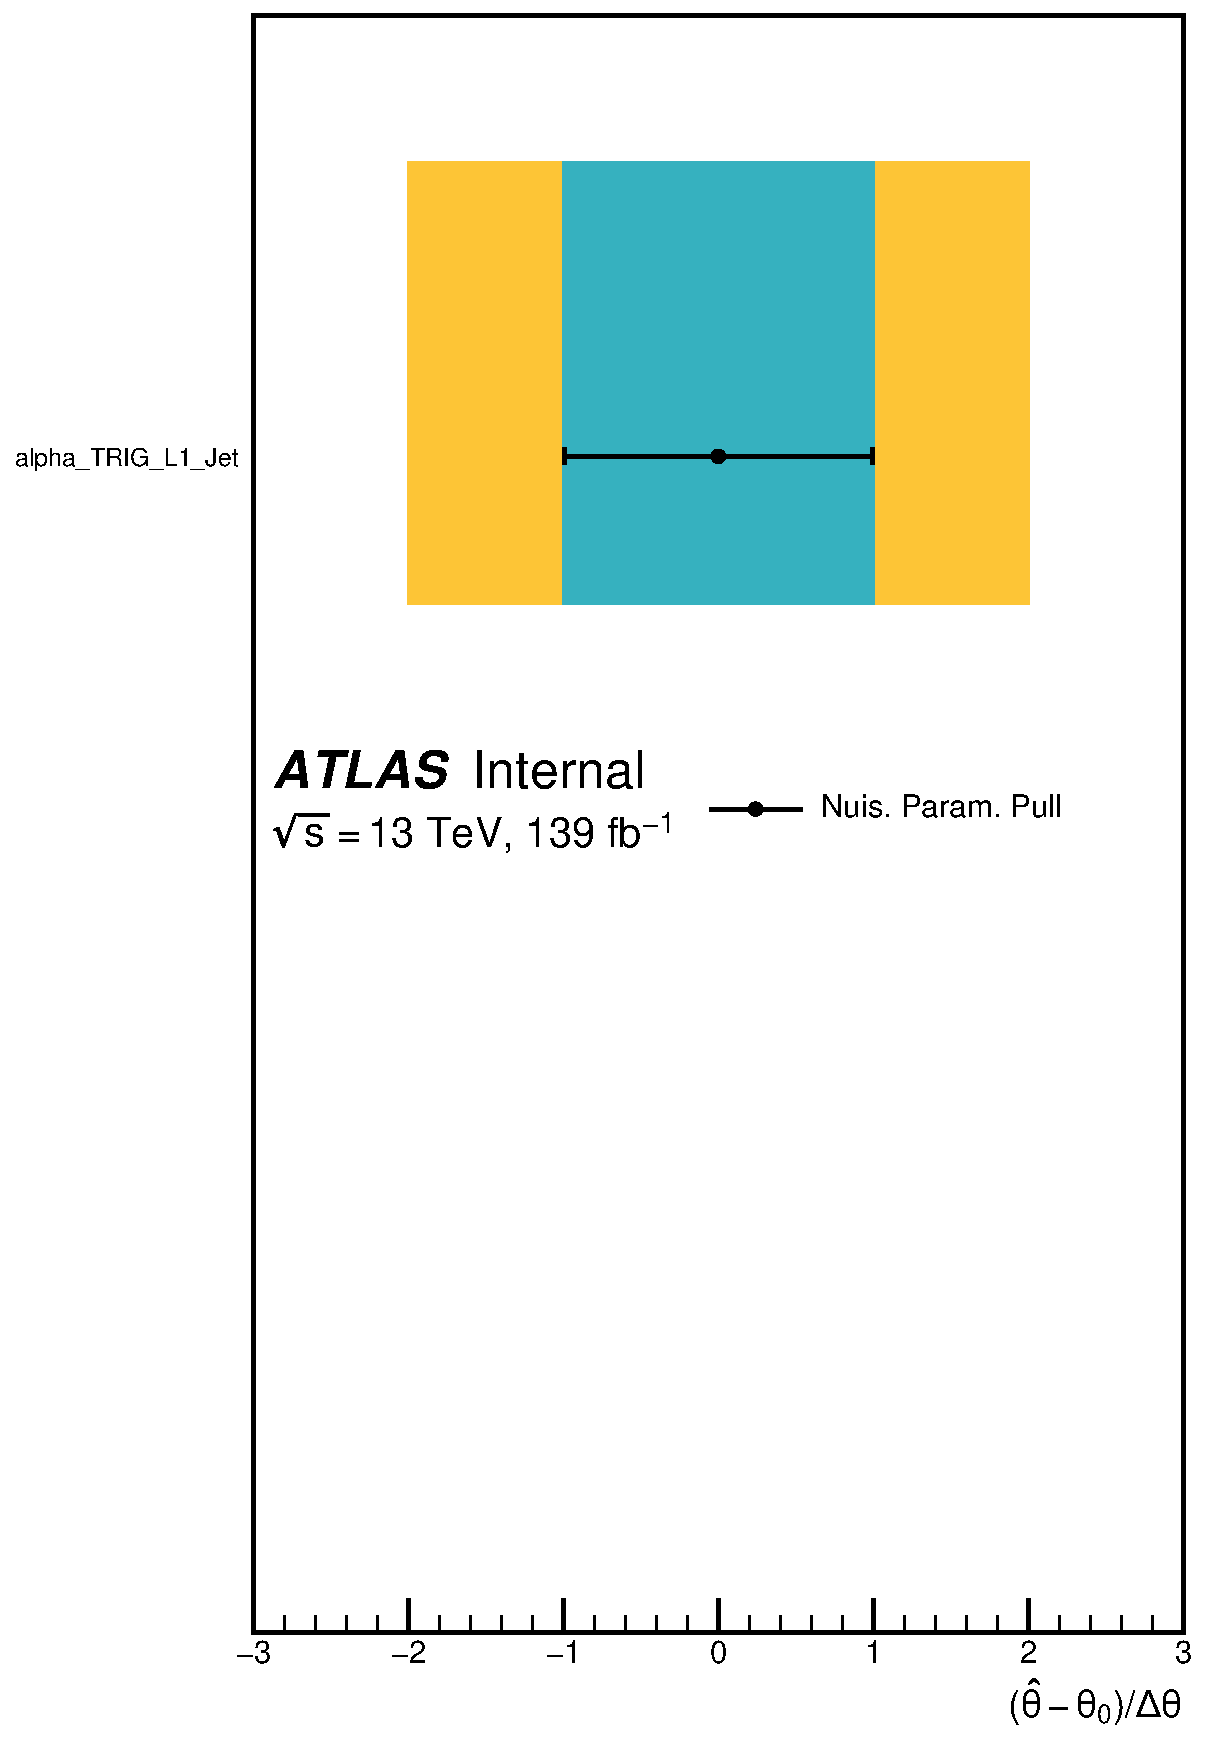
\includegraphics[width=0.33\textwidth]{\figDir/\corrscheme/pulls/quickstats_pulls_correlated_fullsyst_unblind_bkg_new_deta_Xhh_3x2_res_p09_samps_ggf_pd_ggf_161718_mod_kl_1/quickstats_pulls_correlated_fullsyst_unblind_bkg_new_deta_Xhh_3x2_res_p09_samps_ggf_pd_ggf_161718_mod_kl_1.00_k2v_1.00_k1v_1.00_b_only_rank_0001_to_0081_5-end.pdf}	% \caption{Background estimation related NP pulls from a background only (left) or a SM signal + background (right) fit to data in the ggF channel.}
	\caption{NP pulls from a background only fit to data in the ggF channel. Note the theoretical uncertainties on the xsec due to the pdf and mtop unc (`THEO\_XS\_PDFalphas' and `THEO\_XS\_SCALEMTop') are not included in the fit.
	}
	\label{fig:ggf-pulls-corr-bonly}
\end{figure}




\begin{figure}[htp]
\centering
	\includegraphics[width=1\textwidth]{\figDir/\corrscheme/np_correlation/NP_correlation_matrix_correlated_fullsyst_unblind_bkg_new_deta_Xhh_3x2_res_p09_samps_ggf_pd_ggf_161718_mod_kl_1.00_k2v_1.00_k1v_1.pdf}
	\caption{Correlation matrix of NPs from a signal (SM) + background fit to data in the ggF channel.}
	\label{fig:ggf-correlation-matrix-corr-sm}
\end{figure}

Basically we only have non-trivial correlations between the background systematics.


%%%%%%%%%%%%%%%%%%%%%%%%%
% Correlation plot for the combined S+B fit
%%%%%%%%%%%%%%%%%%%%%%%%%

\begin{figure}[htp]
\centering
\subfloat[]{
	\includegraphics[width=1\textwidth]{\figDir/\corrscheme/np_correlation/NP_correlation_matrix_correlated_fullsyst_unblind_ggF_VBF_comb_samps_ggf_and_vbf_pd_ggf_161718_vbf_inc161718_mod_kl_1.00_k2v_1.00_k1v_1.pdf}}
	\caption{Correlation matrix of NPs from a signal + background fit to data in the combined ggF + VBF channel.}
	\label{fig:ggf_vbf-correlation-matrix-corr-sm}
\end{figure}